\documentclass[a4paper,12pt]{article}
\usepackage[utf8]{inputenc} 
\usepackage[T1]{fontenc}
\usepackage{lmodern}
\usepackage{amsmath, amssymb, amsthm}
\usepackage{graphicx}
\usepackage{float}
\usepackage{algorithm}
\usepackage{algorithmic}
\usepackage{caption}
\usepackage{subcaption}
\usepackage{fullpage}
\usepackage{hyperref} % per indici e link cliccabili
\usepackage{booktabs}

\hypersetup{
    colorlinks=true,
    linkcolor=blue,
    urlcolor=blue,
    pdftitle={Relazione sul WFVS con HGA},
    pdfpagemode=FullScreen,
}

\title{Relazione sul Problema del Weighted Feedback Vertex Set\\
utilizzando un Algoritmo Ibrido Genetico (HGA)}
\author{Santi Lisi (1000044181)}
\date{Marzo 2025}

\begin{document}
\maketitle

\tableofcontents
\clearpage

\section{Introduzione}
Il problema del \emph{Weighted Feedback Vertex Set} (WFVS) consiste nel trovare un sottoinsieme di vertici in un grafo, la cui rimozione renda il grafo aciclico, minimizzando la somma dei pesi dei vertici rimossi. Formalmente, dato un grafo $G=(V,E)$ e una funzione di peso $w:V\rightarrow \mathbb{R}^{+}$, l'obiettivo è:
\[
\min_{S\subseteq V} \sum_{v\in S}w(v)
\]
tale che il grafo $G'=(V\setminus S, E')$ sia aciclico.

\subsection{Applicazioni ed Esempio}
Il WFVS viene utilizzato in:
\begin{itemize}
    \item Sistemi operativi, per la prevenzione dei deadlock.
    \item Sistemi distribuiti, per evitare stalli nelle comunicazioni.
    \item Verifica dei programmi e sicurezza informatica.
\end{itemize}

La Figura~\ref{fig:esempio_grafo} mostra un esempio di grafo e la rimozione di vertici per ottenere un grafo aciclico.

\begin{figure}[H]
    \centering
    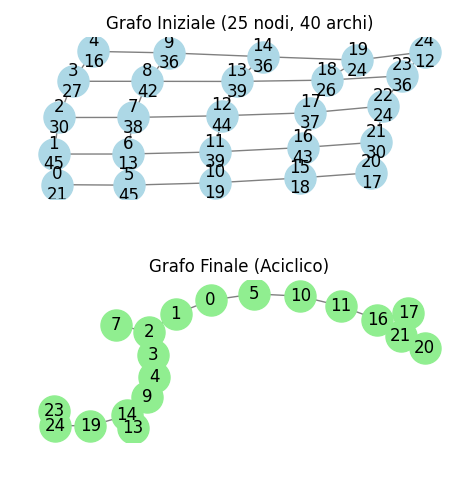
\includegraphics[width=0.6\textwidth]{res/fvs_graphs_sample.png}
    \caption{Esempio di grafo e rimozione dei vertici per ottenere un grafo aciclico. In cui una soluzione del FVS con 25 nodi e 40 archi è: {6,8,12,15,18,22}}
    \label{fig:esempio_grafo}
\end{figure}

\section{Algoritmo Utilizzato}

Per risolvere il problema del \emph{Weighted Feedback Vertex Set} (WFVS) è stato sviluppato un Algoritmo Ibrido Genetico (HGA) che integra operatori evolutivi, una funzione di riparazione e una strategia di ricerca locale. L'approccio scelto è particolarmente efficace per questo problema per i seguenti motivi:

\begin{itemize}
    \item \textbf{Selezione a torneo:} Ad ogni torneo vengono scelti $k$ individui casualmente e si seleziona il migliore, garantendo un equilibrio tra diversità e selezione del meglio.
    \item \textbf{Crossover a un punto:} I genitori vengono suddivisi in un punto casuale, scambiando le rispettive porzioni per generare nuovi individui, facilitando lo scambio di informazioni utili.
    \item \textbf{Mutazione:} La mutazione viene applicata su ogni gene (rappresentante di un vertice della soluzione) con una probabilità fissa (ad esempio, 0.065), garantendo l'esplorazione dell'intero spazio delle soluzioni.
    \item \textbf{Funzione di riparazione:} Se una soluzione genera un grafo che contiene cicli, la funzione di riparazione interviene rimuovendo il vertice con il peso minimo all'interno di un ciclo, assicurando così che il grafo risultante sia aciclico.
    \item \textbf{Ricerca locale:} Viene eseguito un hill climbing basato sul criterio di \emph{best improvement}. In altre parole, viene esplorato un campione casuale dei geni e si accetta il miglior miglioramento possibile, affinando la soluzione in maniera efficace.
\end{itemize}

Questa combinazione consente di bilanciare l'esplorazione globale della popolazione con un affinamento locale accurato, garantendo soluzioni valide e ottimizzate per il problema WFVS.

\subsection{Parametri del HGA}
I parametri dell'algoritmo HGA implementato sono i seguenti:
\begin{itemize}
    \item \textbf{Dimensione della popolazione}: il numero di soluzioni iniziali generate casualmente. Un'ampia popolazione favorisce una migliore esplorazione dello spazio delle soluzioni.
    \item \textbf{Numero di generazioni}: il numero di iterazioni in cui la popolazione viene evoluta. Un numero elevato di generazioni permette un affinamento progressivo, anche se aumenta il tempo di esecuzione.
    \item \textbf{Dimensione del torneo}: il numero di individui selezionati casualmente per determinare il migliore durante la selezione a torneo. Questo parametro bilancia la pressione selettiva con il mantenimento della diversità.
    \item \textbf{Tasso di mutazione}: la probabilità che ogni gene (rappresentante di un vertice) venga invertito. Un valore moderato aiuta a evitare la stagnazione mantenendo la possibilità di esplorare nuove soluzioni.
    \item \textbf{Tasso di crossover}: la probabilità che due individui vengano incrociati per generare figli. Un alto tasso di crossover favorisce lo scambio di informazioni tra le soluzioni, contribuendo a miglioramenti significativi.
    \item \textbf{Dimensione del sottoinsieme per la local search}: il numero di geni scelti casualmente da esplorare durante la ricerca locale (hill climbing). Questo parametro controlla il compromesso tra efficienza computazionale e capacità di affinamento della soluzione.
\end{itemize}
Grazie a questi parametri, l'algoritmo riesce a esplorare efficacemente lo spazio delle soluzioni e a trovare soluzioni progressivamente più ottimali.

\subsection{Pseudocodice dell'Algoritmo Ibrido Genetico}

\begin{algorithm}[H]
\caption{Algoritmo Ibrido Genetico per il WFVS}
\begin{algorithmic}[1]
\REQUIRE Grafo $G$, pesi $w$, costo massimo $maxCost$, dimensione popolazione $pop\_size$, numero di generazioni $G_{max}$
\STATE Inizializza popolazione $P$ con soluzioni casuali
\FOR{ogni soluzione $s \in P$}
    \STATE $s \gets$ \textbf{Ripara}(s)
    \STATE $s \gets$ \textbf{LocalSearch}(s)
\ENDFOR
\FOR{$gen = 1$ \TO $G_{max}$}
    \STATE Valuta la fitness per ogni soluzione in $P$
    \STATE Seleziona genitori tramite \textbf{$k$-tournament}
    \STATE Applica \textbf{Crossover} e \textbf{Mutazione} per generare figli
    \STATE Affina i figli con \textbf{Local Search} (hill climbing best improvement)
    \STATE Aggiorna la popolazione $P$
\ENDFOR
\RETURN la miglior soluzione trovata
\end{algorithmic}
\end{algorithm}

\subsection{Pseudocodice degli Operatori Evolutivi}

\subsubsection{Tournament Selection}
\begin{algorithm}[H]
\caption{Tournament Selection}
\begin{algorithmic}[1]
\REQUIRE Popolazione $P$, fitness $f$, parametro $k$
\STATE Seleziona casualmente $k$ individui da $P$
\STATE \RETURN l'individuo con il valore di fitness minimo
\end{algorithmic}
\end{algorithm}

\subsubsection{One Point Crossover}
\begin{algorithm}[H]
\caption{One Point Crossover}
\begin{algorithmic}[1]
\REQUIRE Genitori $P_1$ e $P_2$
\IF{lunghezza di $P_1$ o $P_2$ $<$ 2}
    \RETURN $P_1$, $P_2$
\ENDIF
\STATE Scegli un punto di taglio $p$ casuale, con $1 \leq p \leq (\text{lunghezza} - 1)$
\STATE \textbf{Child1} $\gets$ primi $p$ geni di $P_1$ concatenati con i restanti geni di $P_2$
\STATE \textbf{Child2} $\gets$ primi $p$ geni di $P_2$ concatenati con i restanti geni di $P_1$
\RETURN \textbf{Child1}, \textbf{Child2}
\end{algorithmic}
\end{algorithm}

\subsubsection{Mutazione}
\begin{algorithm}[H]
\caption{Mutate}
\begin{algorithmic}[1]
\REQUIRE Individuo $I$, tasso di mutazione $r$
\FOR{ogni gene in $I$}
    \IF{numero casuale $<$ $r$}
        \STATE Inverti il gene (se 0 diventa 1, se 1 diventa 0)
    \ENDIF
\ENDFOR
\RETURN l'individuo mutato
\end{algorithmic}
\end{algorithm}

\subsubsection{Ricerca Locale (Hill Climbing con Best Improvement)}
\begin{algorithm}[H]
\caption{Local Search (Hill Climbing Best Improvement)}
\begin{algorithmic}[1]
\REQUIRE Soluzione $s$, grafo $G$, pesi $w$, costo massimo $maxCost$, parametro sample\_size
\STATE $s \gets$ \textbf{Ripara}(s)
\STATE $best \gets s$, $best\_fit \gets$ Fitness$(s)$
\WHILE{esiste un miglioramento}
    \STATE $improved \gets false$
    \STATE Definisci l'insieme degli indici da esplorare (tutti o un campione casuale)
    \FOR{ogni indice $i$ nell'insieme}
        \STATE Crea il vicino $s'$ modificando il gene $i$ in $best$
        \STATE Calcola $new\_fit =$ Fitness$(s')$
    \ENDFOR
    \STATE $s' \gets$ il vicino con il miglior miglioramento (minimo $new\_fit$)
    \IF{$new\_fit < best\_fit$}
        \STATE $best \gets s'$, $best\_fit \gets new\_fit$
        \STATE $improved \gets true$
    \ENDIF
\ENDWHILE
\RETURN $best$
\end{algorithmic}
\end{algorithm}

\subsection{Motivazioni dell'Approccio}
L'approccio HGA è particolarmente adatto al WFVS per le seguenti ragioni:
\begin{itemize}
    \item La selezione a torneo garantisce una buona diversità mantenendo al contempo la pressione evolutiva verso soluzioni migliori.
    \item Il crossover a punto unico favorisce lo scambio di informazioni tra soluzioni, combinando tratti efficaci.
    \item La mutazione, applicata a ogni gene, permette una rapida esplorazione dello spazio delle soluzioni, evitando il rischio di stagnazione.
    \item La funzione di riparazione, insieme alla ricerca locale basata su hill climbing con best improvement, assicura che le soluzioni siano valide (grafo aciclico) e continuamente migliorate.
\end{itemize}

Questo approccio ibrido combina l'esplorazione globale (attraverso operatori evolutivi) con l'ottimizzazione locale, rendendolo particolarmente efficace per un problema complesso come il WFVS.

\newpage
\section{Risultati}
L'algoritmo è stato testato su tutte le istanze fornite, sia di tipo Grid che di tipo Rand. Per ciascuna istanza sono state eseguite 10 iterazioni. Durante l'esecuzione, alcuni parametri evolutivi, quali il tasso di mutazione (0,065), il tasso di crossover (0,8) e la dimensione del sottoinsieme per la local search (0,5), sono rimasti invariati, poiché diversi esperimenti hanno evidenziato che tali valori garantiscono risultati e prestazioni ottimali. Gli altri parametri, come la dimensione della popolazione, il numero di generazioni e la dimensione del torneo, sono stati variabili e ottimizzati in base alla grandezza e alla densità del grafo. I risultati includono curve di convergenza, grafici dei costi finali per iterazione e una tabella riassuntiva.

\subsection{Visualizzazione dei Risultati}
In allegato a questa relazione sono presenti i plot dei risultati ottenuti per tutte le sei tipologie di problemi forniti. Di seguito vengono presentate due immagini esemplificative, organizzate come segue:\\[1ex]
\textbf{Figura~\ref{fig:grafici}} che mostra:
\begin{itemize}
    \item Il grafo iniziale e il grafo finale (dove vengono rimossi i vertici indicati dalla soluzione migliore);
    \item Il grafico di convergenza, ottenuto dalla concatenazione delle curve di costo di tutte le iterazioni;
    \item Il grafico dei costi finali per iterazione.
\end{itemize}

\begin{figure}[H]
    \centering
    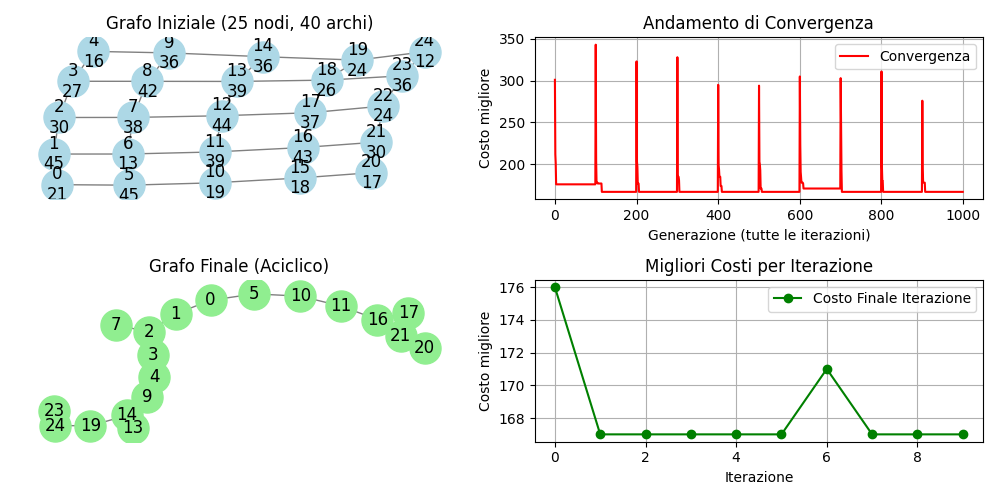
\includegraphics[width=0.9\textwidth]{res/graphs_sample.png}
    \caption{Visualizzazione dei grafici: grafo iniziale, grafo finale, convergenza e costi finali per iterazione.}
    \label{fig:grafici}
\end{figure}

\bigskip

\textbf{Figura~\ref{fig:tabella}} mostra una tabella riassuntiva dei risultati per cinque istanze della stessa categoria (es. Grid), riportando costo minimo, costo medio, deviazione standard, tempo medio e valutazioni.

\begin{figure}[H]
    \centering
    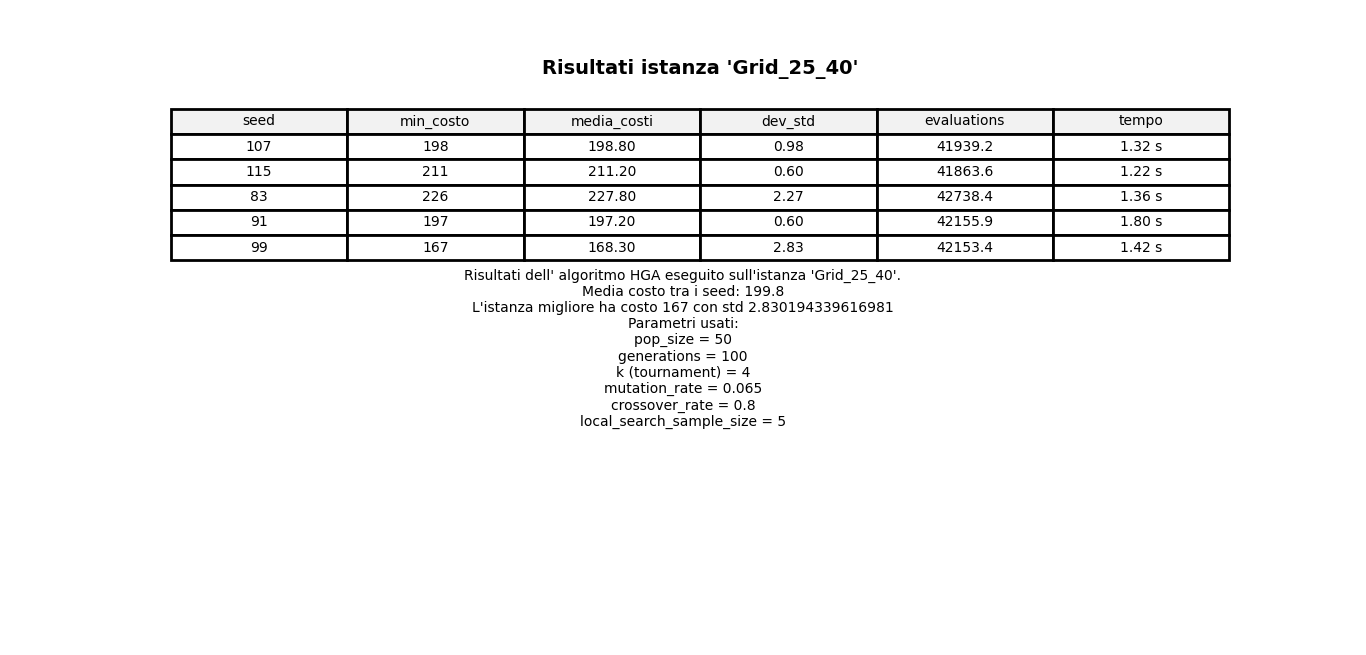
\includegraphics[width=1\textwidth]{res/tab_sample.png}
    \caption{Tabella riassuntiva dei risultati.}
    \label{fig:tabella}
\end{figure}

\bigskip

\textbf{Figura~\ref{fig:zoomConvergence}} illustra il plot dello \emph{andamento di convergenza} zoommato per una singola iterazione di una delle istanze. Questo grafico permette di osservare in dettaglio il comportamento dell'algoritmo durante una singola esecuzione, evidenziando i miglioramenti locali ottenuti.

\begin{figure}[H]
    \centering
    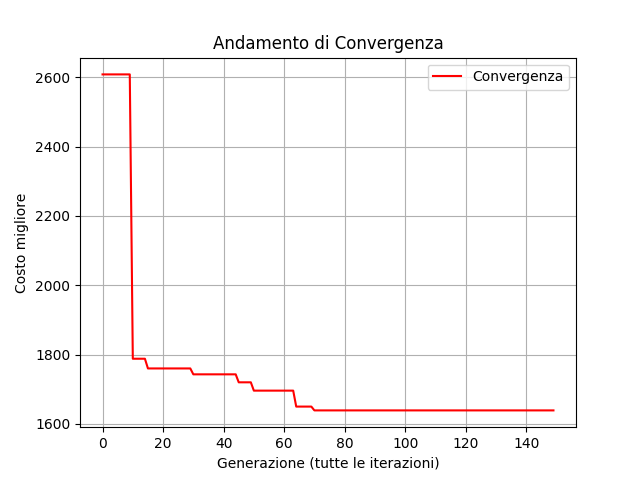
\includegraphics[width=0.7\textwidth]{res/best_interation2.png}
    \caption{Andamento di convergenza zoommato per una singola iterazione.}
    \label{fig:zoomConvergence}
\end{figure}

\subsection{Tabella Riassuntiva dei Risultati Medi e dei parametri usati}
Di seguito una tabella che riassume, per 6 tipi di istanze, la media dei costi, il numero medio di valutazioni e il tempo medio:
\begin{table}[H]
    \centering
    \begin{tabular}{lccc}
    \toprule
    Tipo & PS & G & K \\
    \midrule
    Grid 25\_40 & 50 & 100 & 4 \\
    Grid 49\_84 & 50 & 100 & 4 \\
    Grid 81\_144 & 100 & 150 & 5\\
    Rand 100\_841 & 100 & 150 & 5\\
    Rand 100\_3069 & 250 & 500 & 6\\
    Rand 200\_3184 & 300 & 400 & 8\\
    \bottomrule
    \end{tabular}
    \caption{Parametri usati in ogni istanza: PS = dimensione della popolazione; G = numero di generazioni; K = dimensione del toreno. Altri parametri usati sono: il tasso di mutazione (0.065); tasso di crossover (0.8); la dimensione del sottoinsieme per la local search (5).}
    \label{tab:risultati}
\end{table}
\begin{table}[H]
    \centering
    \begin{tabular}{lccc}
    \toprule
    Tipo & Costo Medio & Valutazioni Medie & Tempo Medio (s) \\
    \midrule
    Grid 25\_40    & 199.8 & 42169.6 & 1.42 s \\
    Grid 49\_84    & 253.2 & 46065.9 & 3.19 s \\
    Grid 81\_144   & 1177.2 & 149182.66 & 16.54 s\\
    Rand 100\_841  & 1759.2 & 141198.76 & 22.35 s\\
    Rand 100\_3069 & 1134.4 & 948675.28 & 141.16 s\\
    Rand 200\_3184 & 5263.0 & 1150266.68 & 465.12 s\\
    \bottomrule
    \end{tabular}
    \caption{Risultati medi trovati per i diversi tipi di istanze.
    Costo Medio: Media dei costi minimi trovati nelle 5 istanze di un ogni tipo; Valutazioni Medie: numero di chiamate medio della funzione di valutazione(fitness) che viene eseguito durante un'iterazione dell'algoritmo HGA su una istanze delle 5; Tempo Medio: Tempo medio (espresso in secondi) che rappresenta la durata di un'iterazione dell'algoritmo HGA su una instanza delle 5.}
    \label{tab:risultati}
\end{table}

\newpage

\section{Conclusioni e Prospettive Future}
L'algoritmo ibrido genetico implementato ha dimostrato efficacia nel risolvere il problema WFVS, ottenendo soluzioni di alta qualità in tempi ragionevoli. In particolare:
\begin{itemize}
    \item La combinazione di operatori evolutivi e la ricerca locale ha accelerato la convergenza .
    \item La funzione di riparazione garantisce che le soluzioni siano sempre valide (grafo aciclico).
    \item I risultati sperimentali mostrano stabilità e performance soddisfacenti.
\end{itemize}


Nonostante i risultati ottenuti con l'algoritmo HGA, sono possibili ulteriori ottimizzazioni che potrebbero portare a performance ancora migliori. Tra le possibili direzioni di ricerca si suggerisce:

\begin{itemize}
    \item \textbf{Ricerca Locale:} 
    \begin{itemize}
        \item Sperimentare con altri metodi di ricerca locale, quali il Simulated Annealing o la Tabu Search, per migliorare l'abilità dell'algoritmo di uscire dai minimi locali.
    \end{itemize}
    \item \textbf{Parametrizzazione:}
    \begin{itemize}
        \item Aumentare o adattare dinamicamente la dimensione della popolazione e il numero di generazioni in funzione della complessità e della densità del grafo.
    \end{itemize}
    \item \textbf{Selezione dei Genitori:}
    \begin{itemize}
        \item Sperimentare altre modalità di selezione, come la selezione a roulette o strategie elitiste, per mantenere una maggiore diversità e garantire un migliore mix delle soluzioni.
    \end{itemize}
    \item \textbf{Crossover:}
    \begin{itemize}
        \item Valutare alternative al crossover a un punto, come il crossover uniforme o multi-punto, per favorire uno scambio più efficace delle informazioni tra i genitori.
    \end{itemize}
\end{itemize}

Queste possibili modifiche potrebbero non solo migliorare la qualità delle soluzioni ottenute, ma anche ridurre i tempi di esecuzione e aumentare la robustezza dell'algoritmo in presenza di istanze particolarmente complesse.

\newpage
\section{Bibliografia}
I riferimenti utilizzati per questo progetto sono stati principalmente le slide del corso, unitamente a fonti online autorevoli. 
\begin{thebibliography}{9}
\bibitem{Slides}
Slide del corso.
\bibitem{GAweb}
"Genetic Algorithms", disponibile su: \url{https://www.sciencedirect.com/topics/computer-science/genetic-algoritahm}.
\bibitem{HillClimbingWeb}
Wikipedia, "Hill climbing", disponibile all'indirizzo: \url{https://en.wikipedia.org/wiki/Hill_climbing} (Accesso: marzo 2025).
\end{thebibliography}
\end{document}
